%
% File acl2018.tex
%
%% Based on the style files for ACL-2017, with some changes, which were, in turn,
%% Based on the style files for ACL-2015, with some improvements
%%  taken from the NAACL-2016 style
%% Based on the style files for ACL-2014, which were, in turn,
%% based on ACL-2013, ACL-2012, ACL-2011, ACL-2010, ACL-IJCNLP-2009,
%% EACL-2009, IJCNLP-2008...
%% Based on the style files for EACL 2006 by 
%%e.agirre@ehu.es or Sergi.Balari@uab.es
%% and that of ACL 08 by Joakim Nivre and Noah Smith

\documentclass[11pt,a4paper]{article}
\usepackage[hyperref]{acl2018}
\usepackage{times}
\usepackage{latexsym}
\usepackage{graphicx}
\usepackage{figsize}

\usepackage{url}

%\aclfinalcopy % Uncomment this line for the final submission
%\def\aclpaperid{***} %  Enter the acl Paper ID here

%\setlength\titlebox{5cm}
% You can expand the titlebox if you need extra space
% to show all the authors. Please do not make the titlebox
% smaller than 5cm (the original size); we will check this
% in the camera-ready version and ask you to change it back.

\newcommand\BibTeX{B{\sc ib}\TeX}

\title{Exploring the effect of dataset on chatbot performance}

\author {Weiting Zhan, Hyein Jeong \\
  University of California, Santa Cruz / Address line 1 \\
  Affiliation / Address line 2 \\
  Affiliation / Address line 3 \\
  {\tt email@domain} \\\And
  Second Author \\
  Affiliation / Address line 1 \\
  Affiliation / Address line 2 \\
  Affiliation / Address line 3 \\
  {\tt email@domain} \\}

\date{May 1, 2019}

\begin{document}
\maketitle
\begin{abstract}
This paper explored the effect of dataset on chat bot performance. The chat bot are trained on Cornell Movie Corpus, Daily Dialog Corpus, and the mix of Cornell Movie Corpus and Daily Dialog Corpus. In order to improve the performance of the chat bot, we trained a Dialog Act Classifier to label Cornell Movie Corpus. Then add Dialog Act as a feature to train the Chat bot. We evaluated the chat bot in (1) grammaticality and (2) naturalness (3) interestingness for a sample of 100 for the three different models. 
\end{abstract}



\section{Introduction}

The use of conversational agents or a ChatBot, which are computer programs using natural language interact with human users, have become a trend in industry given advantages they bring about to our daily life.  The main job they provide is automatic customer services, which reduces a large amount of human labors. Despite of huge attentions paid on the development of a ChatBot, there still some limitations that need to be improved. That is, most of the ChatBot models are designed to respond to questions and generate an appropriate answers in a restricted domain. Thus, the respond generated from the ChatBot is unnatural or not human-like. This is because training datasets for the Chatbot model is insufficient. As an attempt to improve this limitation, we try expanding an existing dataset for the Chatbot model. We implement a pytorch \cite{paszke2017automatic} ChatBot tutorial to Cornell Movie Corpus \cite{Danescu-Niculescu-Mizil+Lee:11a} and Daily Dialogue dataset\cite{li2017dailydialog} individually. Also, we combine the two datasets and apply it to the ChatBot model. 


 
\section{Related work}

Rule-based or template-based methods \cite{williams2016end}, \cite{wen2016network} and dialogue state tracking are typically adopted close-domain systems \cite{henderson2015machine}\cite{wang2013simple}\cite{wen2016network}. In contrast, data-driven techniques such as Seq2Seq generation are used for open-domain chatbots. In general, QA knowledge base or conversational corpus is used to train the Seq2Seq based generation chatbots to generate a response for each input\cite{wu2016sequential}. Several previous works reveal that RNN based Seq2Seq models are suitable for this work \cite{cho2014learning} \cite{sutskever2014sequence} \cite{ritter2011data}\cite{shang2015neural} \cite{sordoni2015neural} \cite{serban2016building}. \cite{sutskever2014sequence} proposed a basic seq2seq model and other works such as \cite{bahdanau2014neural}\cite{sordoni2015neural} \cite{song2016two} \cite{quarteroni2007chatbot} \cite{qiu2017alime} \cite{ghose2013toward} enhanced model with attention, context information and diversified answers. Although lots of work have done, the output of seq2seq generation models tend to be unrelated to input and senseless.  


\usepackage{inputenc}wu2016sequential

\section{Dataset}

\begin{table*}
\centering
\begin{tabular}{1ll}
  Dataset  & number of conversation & dialogue act   \\
  \hline
  Cornell Movie corpus &  220,579  &null  \\
  Daily Dialog &  13,118 &  manually labeled \\
  Cornell + Daily&  233,697 & classifier labeled \\
  
\end{tabular}
\caption{Information of the dataset}
\end{table*}


\subsection{Cornell Movie Corpus}
We use Cornell Movie Corpus, which contains a large collection of fictional conversations extracted from raw movie scripts. To be more specific, it is composed of 220, 579 dialogues between 10,292 pairs of characters in 617 movies, which involve the 9,035 characters. In total, there are 304, 713 utterances in the corpus. Features included in movie metadata are genres, release year, IMDB (Internet Movie Database) rating, and number of IMDB votes. Features of characters metadata include gender (for 3,774 characters) and position on movie credits (for 3,321 characters).

\subsection{Daily Dialog}
We also use Daily Dialogue dataset, which contains 13,118 multi-turn dialogues. This dataset is constructed by crawling the raw data from various websites where English learners practice English dialogue in daily life.  Therefore, this dataset is written by human, which makes it more formal compared to other datasets, such as Twitter Dialog Corpus and Chinese Weibo dataset. Also, Daily Dialogue dataset includes conversations regarding with a certain topic, such as shopping and trips. For example, it includes a conversation between a customer looking for a particular product and a staff at a shop helping the customer. Also, it contains a conversation between two students talking about vacation trips. Moreover, dialogues in this dataset ends after more speaker turns compared to other datasets. That is, the dialogues in Daily Dialogue include in average about 8 turns, but about three topics in other datasets. When it comes to the average, average speaker turns per dialogue is 7.9, average tokens per dialogue is 114.7, and average tokens per utterance is 14.6. 
Also, the Daily Dialogue dataset is manually labeled to reflect intention of communication and human emotions. For intention of communication, which our project is focused on, each utterance in the dataset is labeled with one of four dialogue act classes, that is, Inform, when a speaker is providing information, Questions when a speaker is seeking for information, Directives when a speaker requests, instructs, suggest and accepts or rejects offer, and Commissives when a speaker accepts or rejects a request/suggestion/offer.

\subsection{Mixed dataset}

We first implement a chatbot model to Cornell Movie Corpus and Daily Dialogue dataset individually. In other words, we have a Cornell Movie Corpus, which is a dialogue dataset without a Dialogue Act (DA) label, and Daily Dialogue dataset, which already is already labeled with DA. After deleting DA from Daily Dialogue dataset, we combine Cornell Movie Corpus and Daily Dialogue as one dataset. 



\section{Sequence to Sequence Dialogue Agent}
\begin{figure}
\centering
\SetFigLayout{3}{2}
  \subfigure[Sequence to Sequence model]{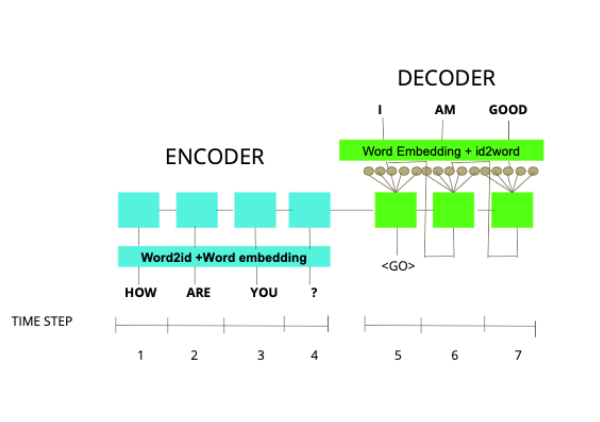
\includegraphics{Fig/SeqtoSeq.png}}
  \hfill
  \subfigure[Sequence to Sequence model and dialog act]{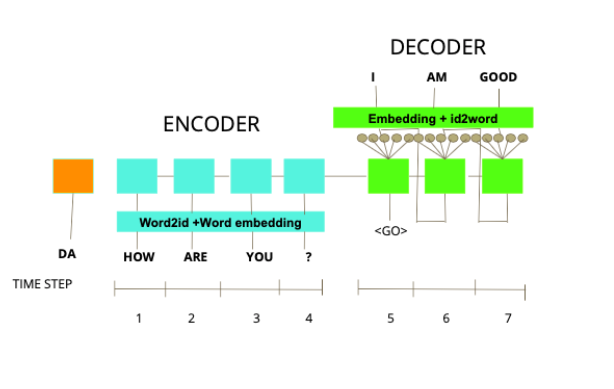
\includegraphics{Fig/Seq2SeqDA.png}}
  \hfill
\caption{Chat bot model}
\end{figure}

\subsection{Data preparation}
Handle loading and preprocessing of Cornell Movie-Dialogs Corpus dataset and daily dialogue dataset.



\subsection{Implement a sequence-to-sequence model with Luong attention mechanism(s)}
Luong attention used top hidden layer states in both of encoder and decoder. In Luong attention they get the decoder hidden state at time t. Then calculate attention scores and from that get the context vector which will be concatenated with hidden state of the decoder and then predict.


\subsection{Jointly train encoder and decoder models using mini-batches}
We built an encoder and decoder recurrent neural network (RNN) with long short-term memory units (LSTM) so that the model can capture word dependencies [15]. The embedding dimension is 300, and the dimensionality of the internal state is set to 512.

\subsection{Implement greedy-search decoding module and beam-search decoding}
A simple approximation is to use a greedy search that selects the most likely word at each step in the output sequence. This approach has the benefit that it is very fast, but the quality of the final output sequences may be far from optimal.

The beam search that expands upon the greedy search and returns a list of most likely output sequences.Instead of greedily choosing the most likely next step as the sequence is constructed, the beam search expands all possible next steps and keeps the k most likely, where k is a user-specified parameter and controls the number of beams or parallel searches through the sequence of probabilities.

\section{Experiment}
\subsection{Chat bot 1}
Chat bot 1 is trained on Cornell Movie dataset. In order to decrease the error, we tried two learning rate, 0.01 and 0.001. The result is shown in Fig \ref{Chatbot1}. Apparently, at learning rate 0.001, the training error and validation error can decrease to as low as 1.2.
\begin{figure}
    \centering
    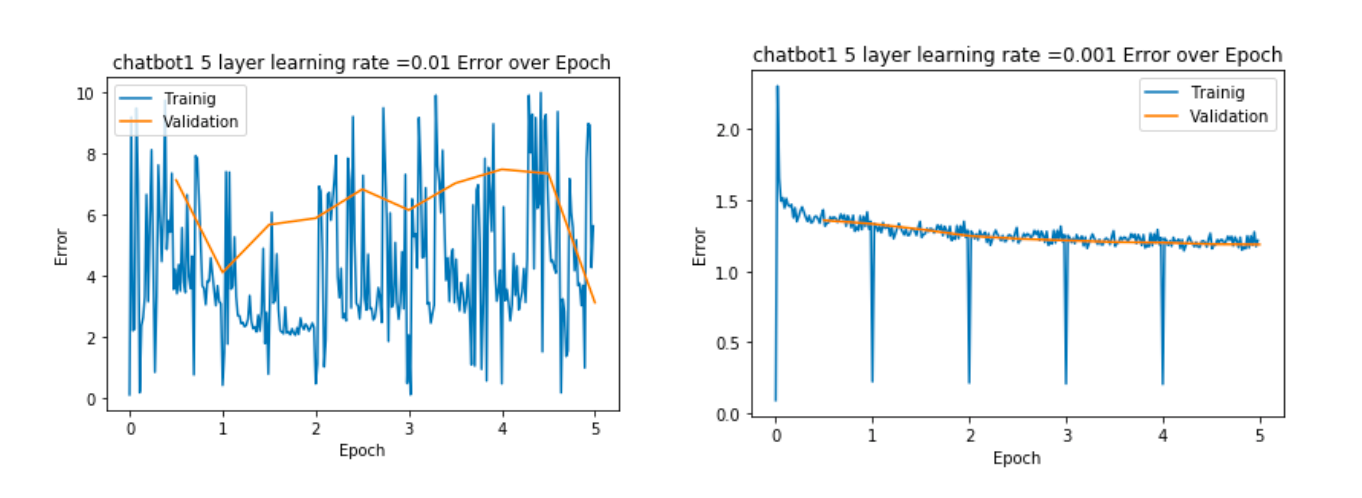
\includegraphics[width =1\linewidth]{Fig/chatbot1.png}
    \caption{Learning rate 0.01 and 0.001 on chat bot 1}
    \label{Chatbot1}
\end{figure}

\subsection{Chat bot 2}
Chat bot 2 is trained on Daily dialogue dataset. As shown in Fig \ref{Chatbot2learningrate}, we conducted our experiment on chat bot 2 with learning rate 0.01 and 0.001. For learning rate 0.01, the training reached 50 epoch, the training error and validation error won't decrease with the increase of epoch. For learning rate 0.001, the error can decrease to 1.2 with only 5 epoch,however, the error stable at 2.6 even trained to 50 epoch at learning rate 0.01. We also increased the number of hidden layer to understanding the model, as shown in Fig \ref{Chatbot2hidden}. 
\begin{figure}
\centering
\SetFigLayout{3}{2}
  \subfigure[learning rate = 0.01]{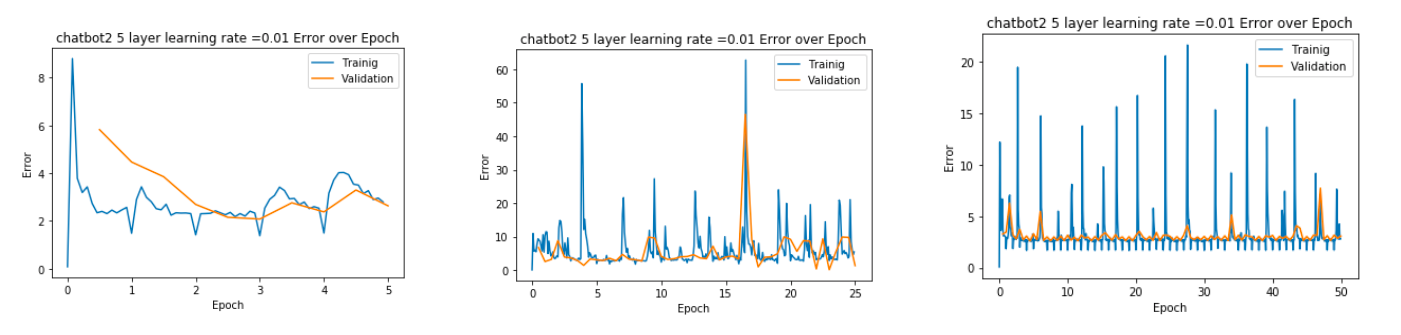
\includegraphics{Fig/chatbot2lR.png}}
  \hfill
  \subfigure[learning rate = 0.001]{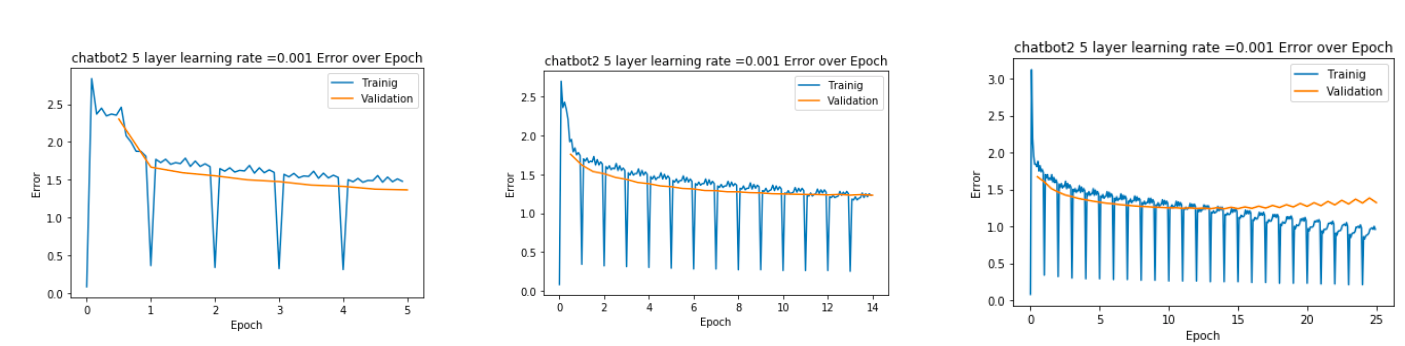
\includegraphics{Fig/chatbot2LR2.png}}
  \hfill
\caption{Learning rate of Chat bot 2}
\label{Chatbot2learningrate}
\end{figure}



\begin{figure}
    \centering
    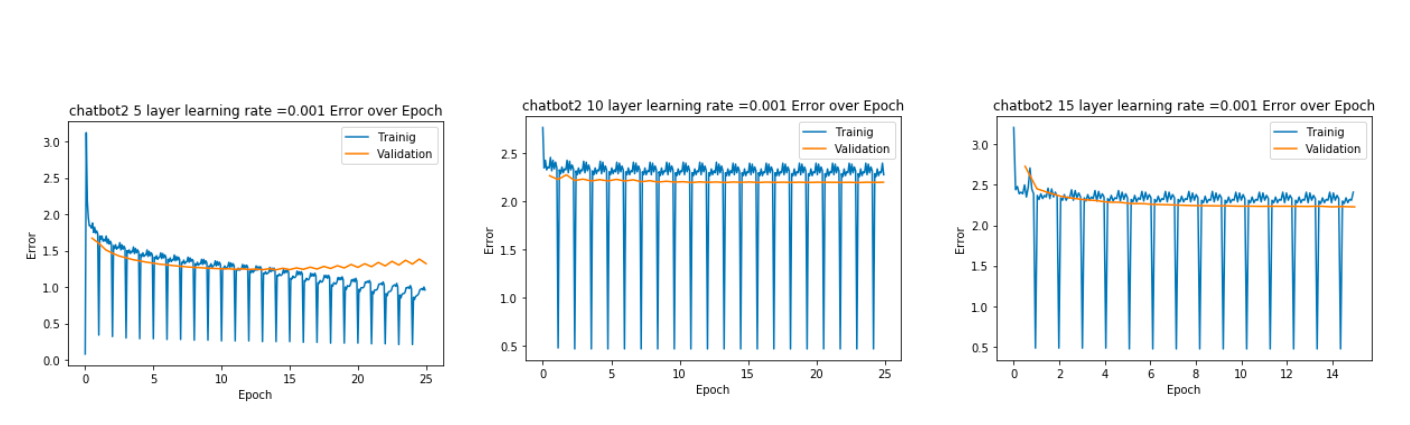
\includegraphics[width =1\linewidth]{Fig/chatbot2layer.png}
    \caption{5,10,15 Hidden layer on chat bot 2 }
    \label{Chatbot2hidden}
\end{figure}

\subsection{Chat bot 3}
Chat bot 3 is trained on the mix of Cornell Movie dataset and Daily Dialogue dataset. We used 0.01 and 0.001 as our learning rate. The learning rate of 0.001 has better performance. In the future, we should explore more learning rate to decrease the error.
\begin{figure}
    \centering
    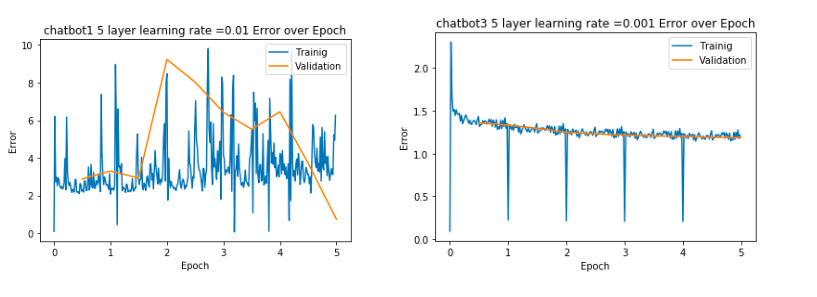
\includegraphics[width =1\linewidth]{Fig/chatbot3.png}
    \caption{Learning rate 0.01 and 0.001 on chat bot 3}
    \label{Chatbot1}
\end{figure}

\begin{table*}
\centering
\begin{tabular}{1lll}
    & Grammaticality &  Naturalness & Interestingness   \\
  \hline
 Chat bot 1, 5 epoch &  3.3 & 2 & 1.7  \\
 Chat bot 2, 5 epoch &  4 &  2.7 & 2.7 \\
 Chat bot 2, 14 epoch &  1 &  1 & 1.7 \\
 Chat bot 2, 25 epoch &  1 & 1 & 2.3 \\
 Chat bot 3, mixed dataset &  3.7 & 4 & 2 \\
  
\end{tabular}
\caption{Average score for each criteria}
\end{table*}

\begin{table}[t!]
\begin{center}
\begin{tabular}{|l|}
\hline \bf 
Hi  \\ 
I am not going to get you to theout.\\
\bf Where are you from?  
\\I am not going to beout.
\\ \bf What do you do for a living?
 \\ I am not going to beout.
\\ \bf Can you let me know what time it is?
 \\I am not going to get out of here.
 \\ \bf Do you have time to go shopping tomorrow?
 \\  I am not going to get aout.
 \\
\bf When is your birthday? \\  
I am not going to get you. \\
\bf Which one do you prefer, a dog or a cat?
\\I am not going to get you to theout. \\
\bf When is the next Olympic?
 \\  I am not going to get you.
 \\
\bf Can you recommend any country to go on & \bf  a trip? 
\\ I am not going to beout.
  \\
\bf How is the weather today?
 
 
 \\  I am not going to get it out of my life.
  \\
\bf I miss my family.
 \\  I am not going to beout.
 \\
\hline
\end{tabular}
\end{center}
\caption{the input and output of chat bot trained with Cornell Movie Corpus}
\end{table}




\begin{table}[t!]
\begin{center}
\begin{tabular}{|l|}
\hline \bf 
Hi  \\ 
I am glad , I am not sure of you ..\\
\bf Where are you from?  
\\I am glad ofout ..
\\ \bf What do you do for a living?
 \\ I am glad , but I will be able to be aout .
\\ \bf Can you let me know what time it is?
 \\I am sorry , but I am not sure ..
 \\ \bf Do you have time to go shopping tomorrow?
 \\  I am glad I will ..
 \\
\bf When is your birthday? \\  
I am sorry , but I am not sure of theout .. \\
\bf Which one do you prefer, a dog or a cat?
\\I am sorry , but I am not sure of you .. \\
\bf When is the next Olympic?
 \\  I am glad , but I am not sure of you ..
 \\
\bf Can you recommend any country to go on & \bf  a trip? 
\\ I am glad of you ..
  \\
\bf How is the weather today?
 
 
 \\  I am sorry , but I am not sure of you ..
  \\
\bf I miss my family.
 \\  I am sorry ..
 \\
\hline
\end{tabular}
\end{center}
\caption{the input and output of chat bot trained with Daily dialogue, 5 epoch. Underfitting result: training error larger than validation error}
\end{table}


\begin{table}[t!]
\begin{center}
\begin{tabular}{|l|}
\hline \bf 
Hi  \\ 
conversation sets awful pardon romance &
brilliant parcel discuss lisa efficient typicalout &
swimming\\
\bf How are you?  
\\conversation sets wilson eaten own & 
conversation level typicalout swimming 
\\ \bf What do you do for a living?
 \\ conversation sets awful romance level &
 pleaseout dance discuss swimming 
\\ \bf Can you let me know what time it is?
 \\conversation sets wilson eaten own & 
however level lisa cameras lisa coach &
western swimming
 \\ \bf Do you have time to go shopping tomorrow?
 \\  conversation sets wilson eaten own & 
owever level lisa cameras lisa coachout &
swimming
 \\
\bf When is your birthday? \\  
conversation sets awful romance maintain &
register swimming
 \\
\bf Which one do you prefer, a dog or a cat?
\\conversation sets awful romance maintain &
register swimming\\
\bf When is the next Olympic?
 \\  conversation sets awful romance maintain &
register swimming\\
\bf Can you recommend any country to go on & \bf  a trip? 
\\  conversation sets awful romance maintain &
register swimming\\
\bf How is the weather today?
\\  conversation sets awful romance maintain &
register swimming\\
\bf I miss my family.
\\  conversation sets awful romance maintain &
register swimming\\

 \\
\hline
\end{tabular}
\end{center}
\caption{the input and output of chat bot trained with Daily dialogue, 14 epoch.Just right result: training error approximately equals to validation error}
\end{table}


\begin{table}[t!]
\begin{center}
\begin{tabular}{|l|}
\hline \bf 
Hi  \\ 
cancer demand charges songs exciting hong &
speed.\\
\bf Where are you from?  
\\cancer demand charges songs magazine & 
palace speed cancer !  cheap santa tend safe&
haven surpriseout speed.
\\ \bf What do you do for a living?
 \\ cancer demand charges songs magazine &
 palace speed cancer ! cheap santa tend safe &
 hospital nice speed.
\\ \bf Can you let me know what time it is?
 \\cancer demand allowed phone independent &
 cancer demand cheap police speed.
 \\ \bf Do you have time to go shopping tomorrow?
 \\  cancer demand allowed phone independent &
 cancer digital certainly safe towards :: &
 definitelyout speed.
 \\
\bf When is your birthday? \\  
cancer demand allowed phone independent &
cancer digital certainly safe towards 
& mexico surprise library speed.
 \\
\bf Which one do you prefer, a dog or a cat?
\\cancer demand allowed phone independent &
cancer demand cheap police whom cancer 
&judge speed. \\
\bf When is the next Olympic?
 \\  cancer demand allowed phone independent &
 cancer digital certainly safe towards mexico &
 definitelyout speed.

 \\
\bf Can you recommend any country to go on & \bf  a trip? 
\\ cancer demand allowed phone independent &
cancer digital certainly safe towards mexico & 
surpriseout speed.

  \\
\bf How is the weather today?
 
 
 \\  cancer demand allowed phone independent &
 cancer digital certainly safe towards mexico songs &
 speed.

  \\
\bf I miss my family.
 \\ cancer demand charges songs certainly surprise &
 wear next speed.

 \\
\hline
\end{tabular}
\end{center}
\caption{the input and output of chat bot trained with Daily dialogue, 25 epoch. Overfitting result: training error less than validation error}
\end{table}







\begin{table}[t!]
\begin{center}
\begin{tabular}{|l|}
\hline \bf 
Hi  \\ 
I am not sure I am not going to be aout.\\
\bf How are you?  
\\I am not sure I am not sure. 
\\ \bf What do you do for a living?
 \\ I am not sure I am not going to be aout.
\\ \bf Can you let me know what time it is?
 \\I am not sure.
 \\ \bf Do you have time to go shopping tomorrow?
 \\  I am not sure I am a littleout.
 \\
\bf When is your birthday? \\  
I am not sure I am not going to be able to be aout.
 \\
\bf Which one do you prefer, a dog or a cat?
\\I am not sure I am not going to be able to be aout.
\\
\bf When is the next Olympic?
 \\ I am not sure. \\
\bf Can you recommend any country to go on & \bf  a trip? 
\\  I am not sure.
\\
\bf How is the weather today?
\\ I am not sure I am not going to be aout.
\\
\bf I miss my family.
\\  I am not sure.
\\

 \\
\hline
\end{tabular}
\end{center}
\caption{the input and output of chat bot trained with mixed dataset, both Cornell Movie Corpus and Daily dialogue.}
\end{table}






\section{Evaluation}


We only conduct  human evaluation to the outputs as it has been debated that it is the only  measure that open-ended generation tasks can rely on \cite{li2016deep}, \cite{wiseman2017challenges}. Indeed, it has been questioned whether automatic  metrics, such as BLEU, are appropriate to capture response quality of open-ended generation tasks \cite{dai2015semi} \cite{galley2015deltableu}.  Considering that open-ended generation does not aim to derive any correct answer, we characterize (1) grammaticality and (2) naturalness (3) interestingness for some samples of the four different models by conducting human evaluation. We asked three people to evaluate each criteria for each model, and average score of each criteria was calculated. Each criteria was evaluated compared to each model.



\subsection{Grammaticality}

For grammaticality, with a scale of 0-5, we evaluate grammatical errors such as whether a model obeys subject verb agreement, whether a model generates a random string of words or a full sentence, and which kind of tense it can generate. 
The chat bot 2, where 5 epoch was used, performs the best in terms of grammaticality. Compared to other models, it generates a grammatical full sentence, which obeys subject verb agreement and can generate future tense. Even if it generates meaningless words, it happens less than other models. Also, it puts a comma and a punctuation mark at the right place. On the other hand, the chat bot 3 performs similar to  the chat bot 2 with 5 epoch, but it misses a punctuation mark between two sentences. Some models, such as chat bot 2 with 25 epoch and with 14 epoch performs not very well as they only generate a random string of words. 

\subsection{Naturalness}

For naturalness, with a scale of 0-5, we evaluate whether a response from a model is similar to natural dialogue. All of the models perform not very well on naturalness as they only repeat either the same string of words or the same sentence. However, the chat bot 3 trained with a mixed dataset was considered as performed the best. This is because for some questions asked to the chat bot, it makes sense to answer with the repetitive sentence that it generates,such as I am not sure.

\subsection{Interestingness}

For interestingness, with a scale of 0-5, we evaluate whether a response from a chat bot evokes a person to continue talking to it. All of the responses generated from each model was not very interesting to continue talking as they all repeat the same sentence or words.  



\section{Conclusion and future work}

We trained chat bots to produce open-ended generation by changing some hyper-parameters, such as epoch, num layers, and learning rate, and reported the results. The biggest problem of the chat bots was that they repeat the same string of words or a sentence. Thus, in order to understand the model better, we need to conduct more experiments on other parameters, such as batch size, rnn size, learning rate decay, min learning rate, and keep probability.





\section*{Acknowledgments}
We are thankful to Prof. Marilyn Walker who provided expertise that greatly assisted the research.

% include your own bib file like this:
%\bibliographystyle{acl}
%\bibliography{acl2018}
\bibliography{acl2018}
\bibliographystyle{acl_natbib}

\end{document}
